En este problema, algoritmo minimax realiza una búsqueda exaustiva en un espacio
de soluciones inmenso, por ello se ha buscado optimizar la representación de los
objetos del problema de cara a la eficiencia del algoritmo.

Los principales objetos son: Piezas y Juego.

\subsection{Piezas}
\label{subsec:piezas}
Cada jugador cuenta con 21 piezas distintas que puede colocar en el tablero con
cualquier rotación, cada una puntúa según el número de casillas que ocupe y sus
esquinas juegan un papel importante puesto que han de colocarse adyacentes a las
de otra pieza del mismo color. Todas estas son características invariantes de
cada pieza que se \textbf{precalculan} al inicio del programa y se guardan en
distintas \textbf{tablas} para poder consultarlas después rápidamente.

\begin{figure}[ht]
	\centering
	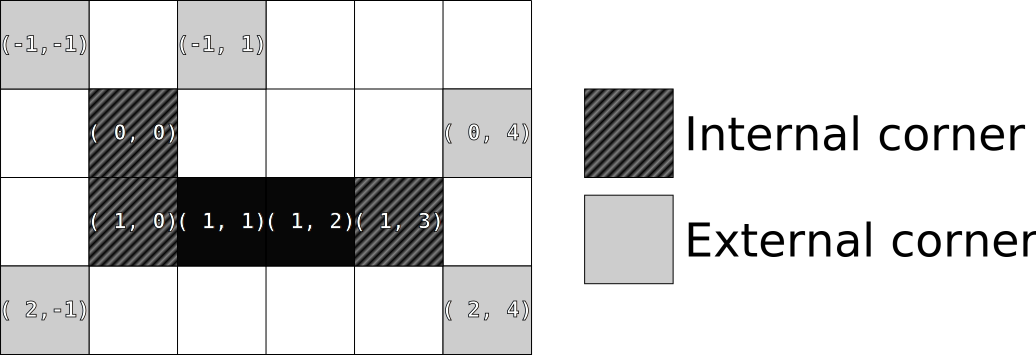
\includegraphics[width=\textwidth, height=0.3\textheight, keepaspectratio]{img/corners}
\end{figure}

Partimos de una lista de piezas creada a mano, \texttt{+btiles+}. Las
piezas están codificadas mediante una matriz donde \texttt{nil} representa una
casilla vacía y \texttt{t} un bloque de la pieza. Esta lista de piezas se ordena
de mayor a menor por puntuación con la intención de que la máquina intente
colocar primero las piezas con mayor puntuación.

A partir de \texttt{+btiles+} creamos todas las tablas:

\begin{itemize}
	\item \texttt{+btiles-points+}: Un vector con las puntuaciones para cada
		tipo de pieza. Se genera a partir de \texttt{+btiles+} y se
		indexa con el identificador de la ficha.

	\item \texttt{+tiles+}: Contiene todas las fichas en forma de matriz de
		\texttt{t - nil} con todas las posibles rotaciones de cada una,
		pero no las rotaciones equivalentes. Se genera a partir de
		\texttt{+btiles+} y se indexa mediante el identificador de la
		ficha y el número de rotación.

	\item \texttt{+tiles-coords+}: Igual que la tabla \texttt{+tiles+}, pero
		las fichas están representadas con una lista de coordenadas
		relativas a su esquina superior izquierda, en lugar de con una
		matrix \texttt{t - nil}. Se genera a partir de \texttt{+tiles+}
		y se indexa de la misma forma.

	\item \texttt{+tiles-external-corners+}: Contiene una lista de las
		``\textbf{esquinas exteriores}'' para cada ficha y para cada
		rotación. Las coordenadas son relativas a la esquina superior
		izquierda de la ficha (pueden ser negativas). Una esquina
		exterior es aquella celda en la que se podría poner una nueva
		pieza: adyacente a una \textsl{esquina interior} pero no a una
		arista. Se genera a partir de \texttt{+tiles-coords+} y se
		indexa por id y rotación.

	\item \texttt{+tiles-internal-corners+}: Similar a
		\texttt{+tiles-external-corners+} contiene las esquinas
		interiores para cada ficha y rotación. Las esquinas interiores
		son aquellos bloques de la pieza que podrían colocarse sobre una
		esquina exterior de otra.
\end{itemize}

Utilidad de cada tabla:
\begin{itemize}
	\item \texttt{+btiles-points+}: Conocer los puntos de cada pieza
		directamente sin necesidad de contar sus bloques cada vez.

	\item \texttt{+tiles+}: Generar fácilmente \texttt{+tiles-coords+}
		entre otros usos menores.

	\item \texttt{+tiles-coords+}: Una lista de coordenadas ahorra
		recorrer casillas vacías cuando se analiza una pieza, a la vez
		que facilita la creación de las tablas de esquinas.

	\item \texttt{+tiles-external-corners+} y
		\texttt{+tiles-internal-corners+}: Suponen una mejora muy
		significativa en la generación de movimientos válidos. Las
		esquinas exteriores permiten conocer las celdas candidatas dónde
		un jugador podría colocar una pieza, mientras que las interiores
		facilitan la colocación de la misma en todas sus posiciones.
\end{itemize}

Con la implementación de las tablas de esquinas se consiguió una mejora en el
rendimiento del algoritmo del \textbf{15000\%}, pasando de tardar \textbf{40
minutos} en tomar una decisión con profundidad 3, a solo \textbf{16 segundos}.

\subsection{Juego}

Para la representación del estado del juego se ha elegido una doble estructura
sincronizada:

\begin{itemize}
	\item Un \textbf{array} de $20 \times 20$ que guarda en casilla id del
		jugador cuándo está ocupada por ese jugador, y \texttt{nil} en
		otro caso.
	\item Una \textbf{lista} de objetos \texttt{player} que contienen, entre
		otros atributos, dos vectores: fichas jugadas
		(\texttt{added-tiles}) y fichas sin jugar (\texttt{held-tiles}).
		Cada una de estas fichas (\texttt{tile}) guarda información
		sobre su posición y rotación.
\end{itemize}

Las ventajas de esta doble estructura son varias. La matriz nos permite
comprobar el estado las celdas vecinas a una dada con un orden constante,
mientras que la listas del jugador nos permite conocer las piezas que ha jugado
y las que no, además de facilitarnos la eliminación de una pieza específica. El
poder añadir y eliminar piezas del tablero es la base de las funciones
\texttt{do-movement} y \texttt{undo-movement}, que suponen un sustancial ahorro
de tiempo y memoria en el algoritmo minimax.
